\documentclass{article}
\usepackage[utf8]{vietnam}
\usepackage{graphicx}
\usepackage{amsmath}
\usepackage{amssymb}
\usepackage{hyperref}
\usepackage{caption}
\usepackage{subcaption}

\title{A gentle introduction to Spatial Filtering. \\ \large Report Lab week 3-4.}
\author{Ngọc Thuận - IPSAL LAB}
\date{18, December 2022}

\begin{document}
\maketitle
\begin{abstract}
    Bài trước chúng ta đã đề cập đến các biến đổi trên miền không gian, và đã tiếp cập với một số phép biến đổi cơ bản trực tiếp lên điểm ảnh (Intensity transformation). Bài này chúng ta sẽ tiếp tục về các phép biến đổi trên miền không gian, cụ thể là phần còn lại (Spatial Filtering). Dưới đây là đôi nét cơ bản về lọc không gian và một số phép lọc cơ bản, đồng thời cũng là phần báo cáo Lab tuần của tôi!
\end{abstract}
\tableofcontents
\newpage
\section{Giới thiệu về lọc không gian}
    \subsection{Chung chung}
    Ta có thể hiểu một bộ lọc không gian gồm hai thành phần:
    \begin{enumerate}
        \item Lân cận (\textit{neighborhood})
        \item Toán tử (\textit{predefined operation})
        
    \end{enumerate}
    Bộ lọc sẽ tạo ra một pixel mới với tọa độ trùng với tọa độ tâm của \textit{neighborhood} và giá trị là kết quả của toán tử. \\ \\    
    Phân loại dựa trên \textit{predefined operation} ta có thể phân loại thành:
    \begin{itemize}
        \item Bộ lọc tuyến tính (\textit{Linear spatial filter})
        \item Bộ lọc phi tuyến tính (\textit{NonLinear spatial filter})
    \end{itemize}
    \underline{\textit{Lưu ý}}: Trong giới hạn bài này ta chỉ làm việc với bộ lọc tuyến tính!\\ \\
    Thông thường khi nhắc tới \textit{Linear spatial filter} của một bức ảnh kích thước \textit{M $\times$ N} với bộ lọc có kích thước \textit{m $\times$ n} ta sẽ hiểu là:
    \begin{equation}
    g(x,y) = \sum_{s=-a}^{a}\sum_{t=-b}^{b} w(s,t)f(x+s,y+t)
    \label{eq1}
    \end{equation}

    x, y thay đổi khi \textit{w} đi qua từng \textit{pixel} trong \textit{f}.
    \\Hình \ref{fig1} cho thấy cách làm việc của bộ lọc tuyến tính!
    \begin{figure}
        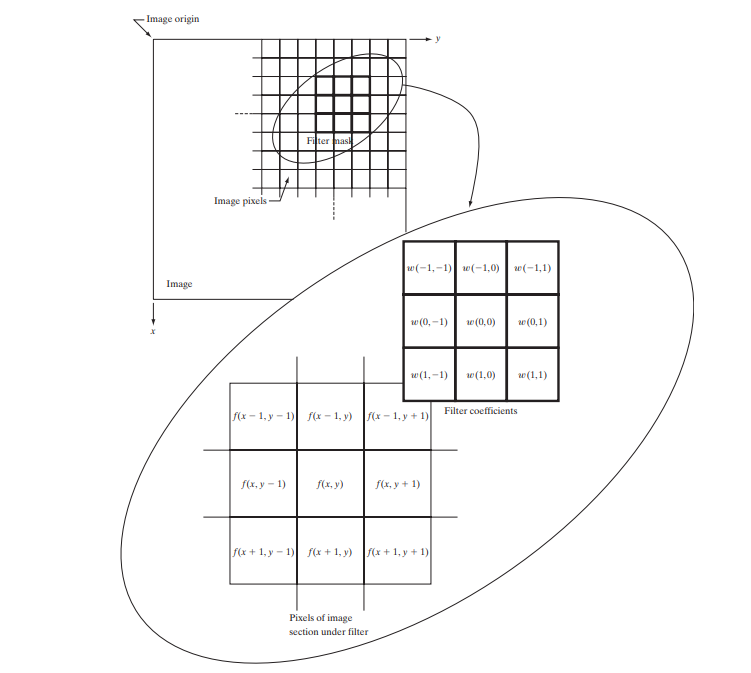
\includegraphics[width = \linewidth]{figure3_28.png}
        \caption{The mechanics of linear spatial filtering using a filter mask. The form chosen to denote the coordinates of the filter mask coefficients simplifies writing expressions for linear filtering}
        \label{fig1}
    \end{figure}
    \newpage
    \subsection{Spatial Correlation and Convolution}
    Đây là hai phép toán quan trọng, nhưng dễ gây nhầm lẫn.
        \subsubsection{Tương quan - Correlation}
        \textit{Correlation } của bộ lọc \textit{w(x,y)} có kích thước \textit{m x n} với ảnh \textit{f(x,y)} được kí hiệu là:
        $$w(x,y) \otimes f(x,y) = \sum_{s=-a}^{a}\sum_{t=-b}^{b} w(s,t)f(x+s,y+t)$$
        \subsubsection{Tích chập - Convolution}
        Khá giống định nghĩa tích chập trong giải tích, 
        $$(f \ast g)(t):=\int_{-\infty}^{\infty} f(\tau) g(t-\tau) d \tau$$
        Trong trường hợp rời rạc,
        $$(f \ast g)[n]=\sum_{m=-\infty}^{\infty} f[m] g[n-m]$$
        \textit{Convolution} của bộ lọc \textit{w(x,y)} có kích thước \textit{m x n} với ảnh \textit{f(x,y)} được kí hiệu là:
        $$w(x,y) \ast f(x,y) = \sum_{s=-a}^{a}\sum_{t=-b}^{b} w(s,t)f(x-s,y-t)$$
        \\ \\
        Hai phép toán trên thật ra cũng không khác nhau nhiều lắm, để có được một trong hai, rõ ràng ta chỉ cần đảo bộ lọc của thằng còn lại. Nên thuật ngũ 'Tích chập' được dùng chung chung cho cả hai, và điều này đôi khi gây nhầm lẫn.\\ \\
        \underline{\textit{Lưu ý:}} Trong phạm vi bài này ta sẽ dùng (\ref{eq1}). Và tôi sẽ dùng thuật ngữ `tích chập' chung cho tất cả các bộ lọc tuyến tính

        \subsection{Tích chập hai chiều - Two dimensional Convolution (2D Convolution)}
        Trước khi đi vào xử lí ảnh, ta sẽ lướt sơ qua về kiểu dáng và cách làm việc với tích chập.
            \subsubsection{Tích chập một chiều}
            Giả sử ta có đầu vào và bộ lọc lần lượt là $\textbf{a} \in \mathbb{R}^{N}$ và $ \textbf{w} \in \mathbb{R}^{f}$ (\textit{f} là số tự nhiên bất kì, thường là số lẻ). Khi đó đầu ra là một vector \textbf{y} với từng phần tử được tính bởi
            $$ y_{n} = \sum_{i=0}^{f-1} a_{n+i}w_{i}$$
            Quá trình đó có thể được thực hiện như sau:
            \begin{enumerate}
                \item Đặt bộ lọc \textbf{w} vào vị trí tương ứng với \textit{f} phẩn tử đầu tiên của \textbf{a}.
                \item Nhân từng phần tử tương ứng của \textbf{w} với \textbf{a} rồi cộng các kết quả lại để được phần tử tương ứng của \textbf{y}.
                \item \textit{Trươt} bộ lọc \textbf{w} một bước sang bên phải. Nểu phần tử cuối cùng của bộ lọc không vượt ra ngoài phần tử cuối cùng của tín hiệu, quay lại Bước 2. Ngược lại, dừng tính toán.
            \end{enumerate}
            \begin{figure}[ht!]
                \centering
                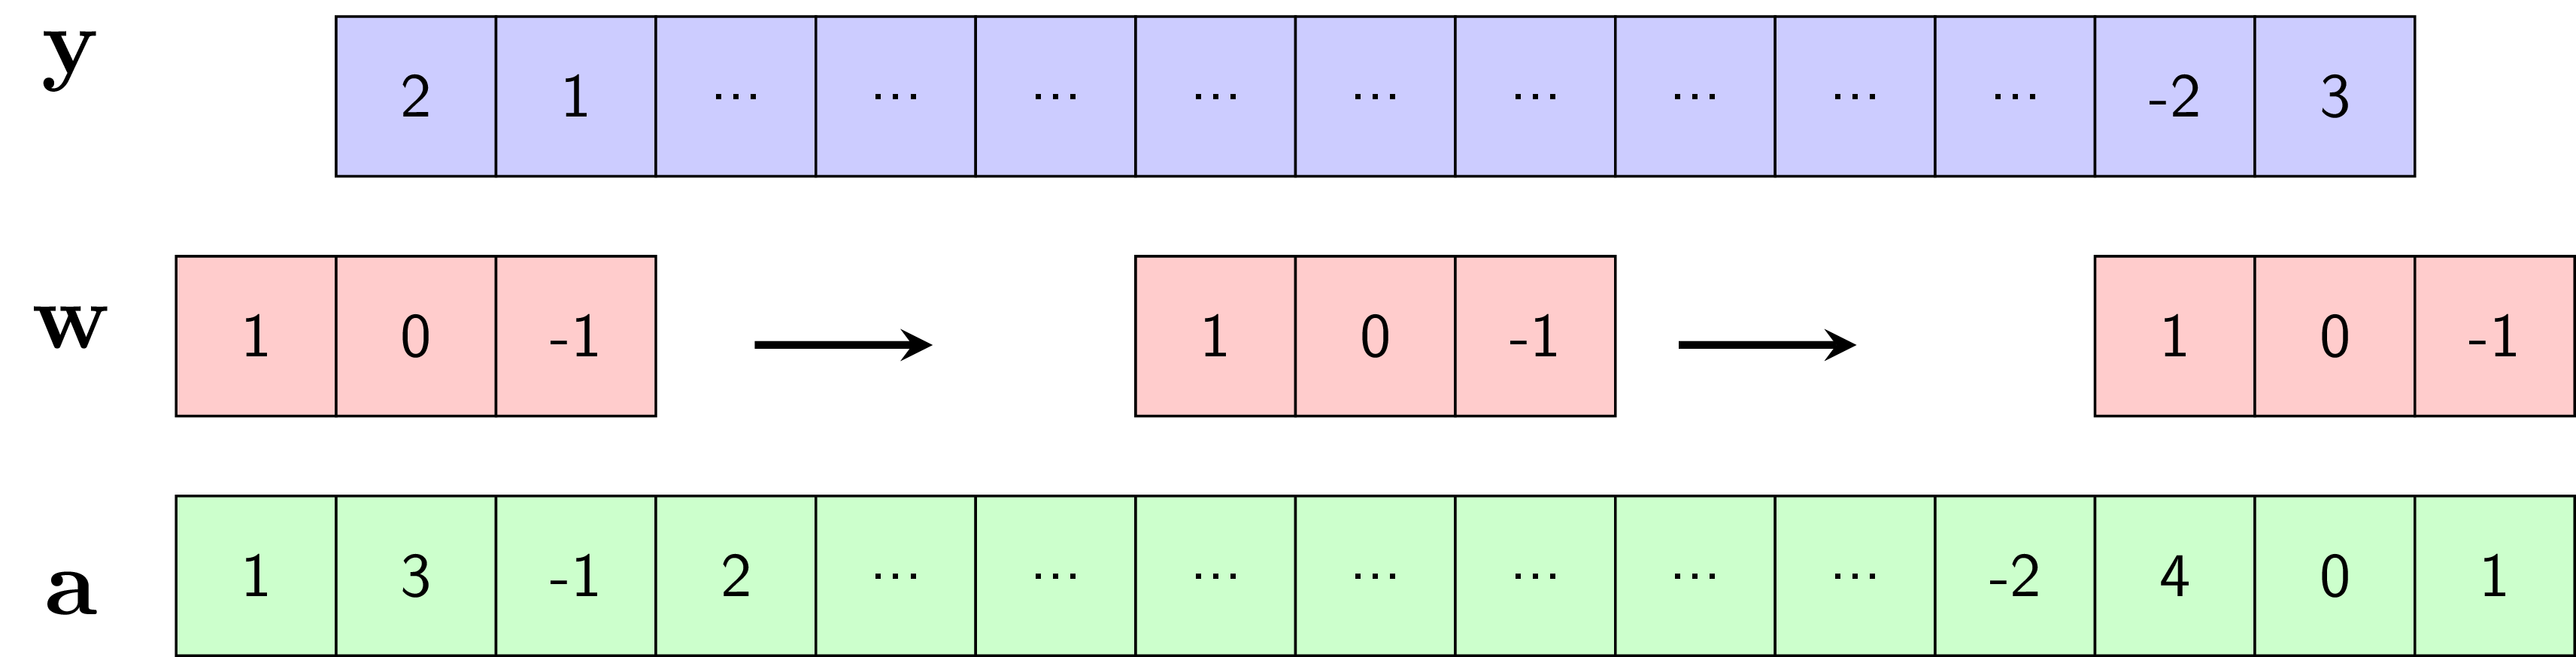
\includegraphics[width = 0.7\linewidth]{conv1d_viz.png}
                \caption{Cách tính tích chập một chiều, machinelearningcoban.com}
                \label{fig2}
            \end{figure}
            Trong ví dụ Hình \ref{fig2}
            $$ y_{0} = a_{0}w_{0}+a_{1}w_{1}+a_{2}w_{2} = 1 - (-1) = 2$$
            $$ y_{1} = a_{1}w_{0}+a_{2}w_{1}+a_{3}w_{2} = 3-2 = 2$$
            Ngoài ra, ta còn hai bước quan trọng khác, có thể cần chú ý là \textit{'Bước trượt - Stride'} và \textit{'Thêm lề - Padding'}, các bạn có thể tham khảo thêm tại: \\ \href{https://machinelearningcoban.com/2018/10/03/conv2d}{Bài 37: Tích chập hai chiều - machinelearningcoban.com}
            \subsubsection{Tích chập hai chiều}
            Là cái ta đã nói ở trên, về cơ bản là tương tự như tích chập một chiều, bộ lọc trượt khắp tín hiệu hai chiều đầu vào theo thứ tự từ trái qua phải, từ trên xuống dưới. Tại mỗi vị trí, các giá trị của bộ lọc và đầu vào tương ứng được nhân với nhau rồi cộng vào lại để thu được kết quả đầu ra.\\
            \begin{figure}
                \centering
                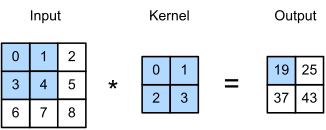
\includegraphics[width = 0.5\linewidth]{correlation.png}
                \caption{Minh họa tích chập hai chiều, diveintodeeplearning}
                \label{fig3}
            \end{figure}
            Giới hạn ở bài này, tôi chỉ dừng lại ở ví dụ về tích chập hai chiều đơn kênh, SISO. Nếu muốn tham khảo thêm các bạn có thể truy cập link bên trên.\\
            Hình \ref{fig3} minh họa cho cách tính tích chập hai chiều.
        \subsection{Thiết kế bộ lọc}
        \label{1}
        Đây không phải là vấn đề gì lớn, nhưng tôi muốn nhắc lại một tí kiến thức về giải tích và phần trước.\\ \\
        Chúng ta biết rằng, trong xử lí ảnh, tín hiệu đầu vào của ta là ảnh số, trong đó giá trị của ảnh được thể hiện qua \textit{pixel}, và tùy thuộc vào lượng \textit{bit} được sử dụng mà giá trị của một điểm ảnh có thể thuộc vào những khoảng khác nhau. Và việc sử dụng một bộ lọc không gian có thể dẫn đến thay đổi những giá trị điểm ảnh, điều đó có thể sẽ khiến kết quả không được như mong muốn. \\ \\
        Để giải quyết việc đó, ta nhắc lại một kết quả quen thuộc trong môn giải tích: \\ \\
        \fbox{
        \begin{minipage}{\textwidth}Giả sử \textit{f(x)} liên tục trên $[a,b]$, có $\alpha + \beta = 1$, $\alpha, \beta$ không âm , khi đó: Tồn tại một số $c \in [a,b]$ thỏa mãn:
        $$ f(c) = \alpha f(a) + \beta f(b)$$
        \end{minipage}}
        \\ \\
        \underline{Chứng minh}\\
        Đặt $\alpha f(a) + \beta f(b) = \mu$. \\
        Do $0 \leq \alpha, \beta \geq 1$, suy ra $\mu \leq max_{[a,b]} f(x)$ và $\mu \geq min_{[a,b]} f(x)$ (*)\\
        Mà, $f(x)$ lại liên tục suy ra $ c \in [c, d]$ với $c, d$ là  argmin, argmax $f(x)$, hiển nhiên $ [c, d] \subset [a, b]$.\\
        Từ đó ta có điều phải chứng minh! \\  \textbf{$\square$ Q.E.D.}
        \\ \\Trên là một kết quả hay và quan trọng. Nhưng ở đây (*) là cái chúng ta cần! \\
        \underline{\textit{Kết luận:}} Mỗi bộ lọc, để đảm bảo đầu ra, cần chuẩn hóa sao cho tổng các phần tử của bộ lọc là bằng 1. \\
        \textit{Chúng ta sẽ thấy rõ điều này ở mục \ref{2} Gaussian Filter - bộ lọc Gauss}\\ \\
        Hình \ref{fig4} ví dụ cho một số bộ lọc hai chiều! 
        \begin{figure}[ht!]
            \centering
            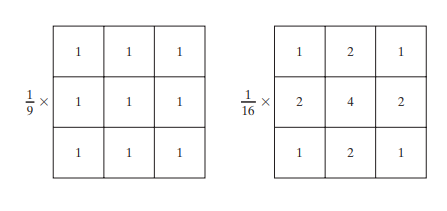
\includegraphics[width = 0.7\linewidth]{fig4.png}
            \caption{Hai bộ lọc làm mịn 3 x 3}
            \label{fig4}
        \end{figure}
    \section{Smoothing Spatial Filters}
    Dịch ra tiếng việt là bộ lọc không gian làm mịn, nghe cứ kì kì.\\ \\
    Đầu ra của bộ lọc không gian làm mịn tuyến tính chỉ đơn giản là trung bình (có trọng số) của các pixel trong vùng lân cận được xác định bởi bộ lọc. Dễ thấy rằng việc này sẽ làm mờ đi cạnh và làm mất đi nhiều chi tiết nhỏ của ảnh.\\ 
    Trọng số ở đây, có thể hiểu là càng gần \textit{center} giá trị càng lớn.\\ \\
    Có một vài bộ lọc khá phổ biến, ví dụ như Hình \ref{fig4}, cho kết quả khá ổn.\\
    \begin{figure}[ht!]
        \centering
        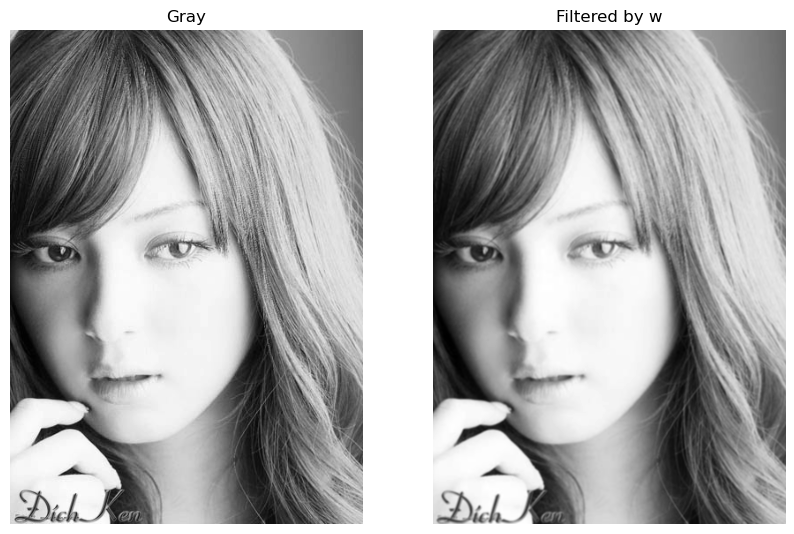
\includegraphics[width = 0.8\linewidth]{download.png}
        \caption{Ảnh xám với bộ lọc bên phải Hình \ref{fig4}}
        \label{fig5}
    \end{figure}
    \begin{figure}[ht!]
        \centering
        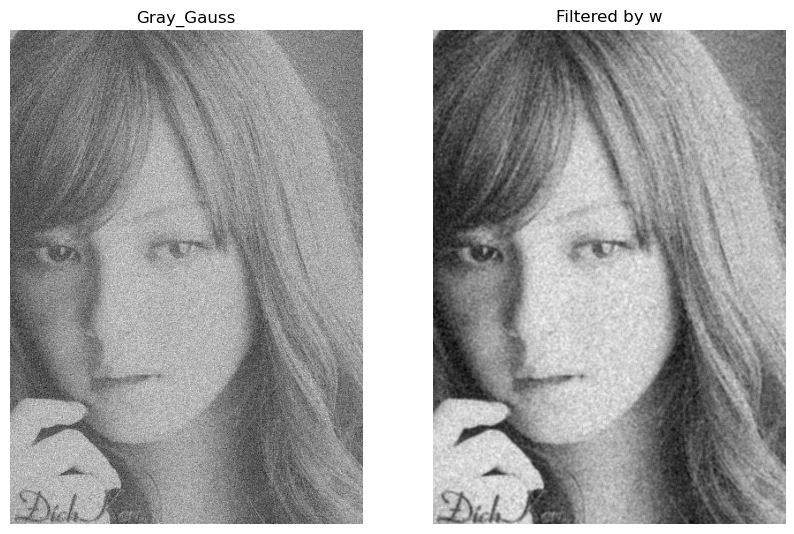
\includegraphics[width = 0.8\linewidth]{download (1).png}
        \caption{Ảnh xám + nhiễu, sử dụng bộ lọc bên trái Hình \ref{fig4}}
        \label{fig6}
    \end{figure}
    Hình \ref{fig5} là minh họa cho bộ lọc bên phải Hình \ref{fig4}. Tuy nhiên với kích thước bộ lọc khá nhỏ ta không thấy rõ, sự khác biệt, Hình \ref{fig6} cho ta một cái nhìn rõ ràng hơn, cũng như cho ta thấy một công dụng khác của bộ lọc không gian là 'khử nhiễu'.

    \subsection{Gaussian Filter}
    \label{2}
    \subsubsection*{Phân phối chuẩn nhiều chiều - Phân phối chuẩn hai chiều}
    Phân phối chuẩn nhiều chiều (\textit{Multivariate Normal Distribution}), giả sử là \textit{D} chiều, \textit{Vector kì vọng} \textbf{$\mu$} và \textit{Covariance matrix $\Sigma$}
    \begin{equation}
        p(\textbf{x}|\textbf{$\mu$}, \textbf{$\Sigma$}) = \frac{1}{(2\pi)^{D/2} {|\textbf{$\Sigma$}|^{1/2}}} \exp{ \left( - \frac{1}{2} \left( \textbf{x} - \textbf{$\mu$} \right)^{T} {\textbf{$\Sigma$}}^{-1} \left( \textbf{x} - \textbf{$\mu$} \right) \right) }
        \label{eq2}
    \end{equation}
    Tuy nhiên, trong ảnh đơn kênh, ta chỉ cần dùng đến 2 chiều, hơn nữa, bộ lọc ta coi trọng số, khoảng cách từ lân cận đến tâm bằng nhau nếu có cùng khoảng cách. Do đó các hệ số tương quan đều bằng 0, và hai chiều có cùng phương sai ${\sigma}^{2}$. Khi đó phương trình (\ref{eq2}) có thể viết lại như sau:
    \begin{equation}
        G(x,y) = \frac{1}{2\pi{\sigma}^{2}} \exp{ \left(- \frac{x^2+y^2}{2{\sigma}^{2}} \right) }
    \end{equation}
    \begin{figure}[ht!]
        \centering
        \begin{subfigure}[b]{0.4\textwidth}
            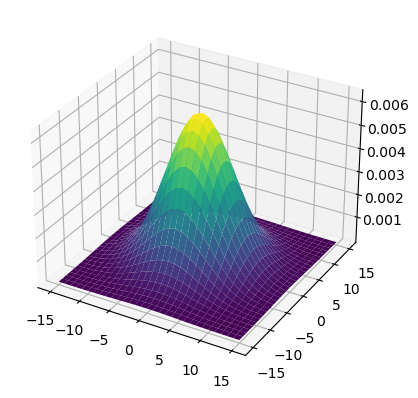
\includegraphics[width = \textwidth]{download (2).png}
            \caption{Đồ thị của phân phối chuẩn hai chiều, ${\sigma} = 5$}
        \end{subfigure}
        \hfill
        \begin{subfigure}[b]{0.4\textwidth}
            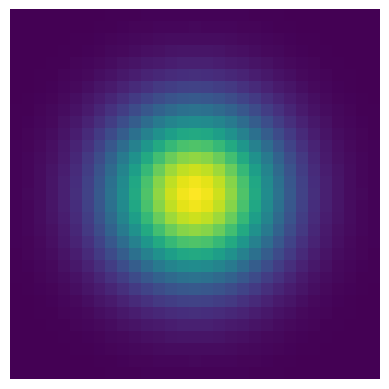
\includegraphics[width = \textwidth]{download (3).png}
            \caption{Kernel, 31 x 31}
        \end{subfigure}
        \caption{Phân phối chuẩn hai chiều}
        \label{fig7}
    \end{figure}
    Hình \ref{fig7} minh họa cho phân phối chuẩn hai chiều trong không gian.

    \newpage
    \subsubsection*{{Quy tắc 3 sigma - \textit{three sigma rule}}}
    \begin{figure}[ht!]
        \centering
        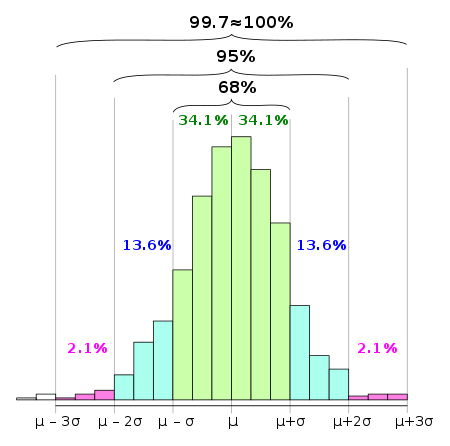
\includegraphics[width = 0.7\linewidth]{thre.png}
        \caption{Quy tắc 3 sigma, wikipedia}
        \label{fig8}
    \end{figure} 
    Hình \ref{fig8} minh họa cho quy tắc 3 sigma, bạn có thể thấy, $P(|x-\mu|<3\sigma) = 99.7\% $ xấp xỉ 1. Theo nhận xét ở mục \ref{1} ta rút ra được cách chọn kích thước bộ lọc: $size = (6n+1, 6n+1)$
    \begin{figure}[ht!]
        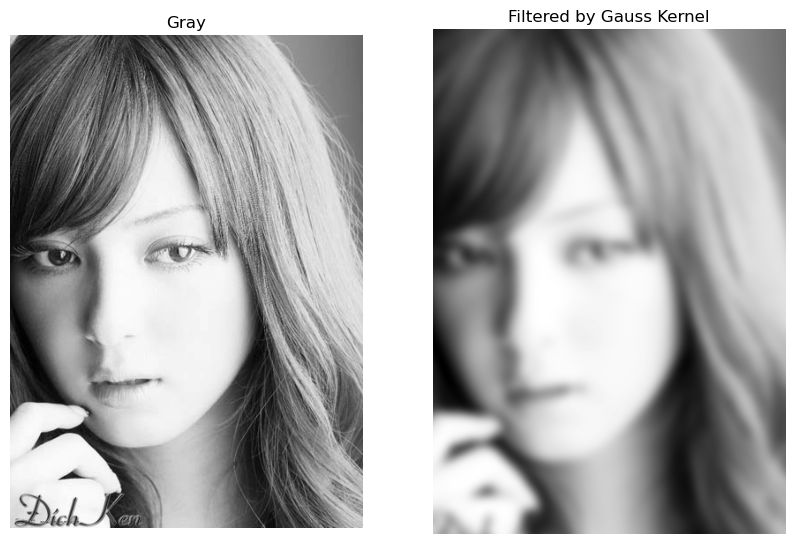
\includegraphics[width = \linewidth]{download (4).png}
        \caption{Làm mờ sử dụng bộ lọc Gauss với bộ lọc Gauss trong Hình \ref{fig7}}
        \label{fig9}
    \end{figure}  
    \\ Hình \ref{fig9} cho thấy kết quả của bộ lọc Gauss.
    \subsubsection*{Khử nhiễu}
    Như nhận xét trên, dẫu biết có thể sử dụng bộ lọc Gauss để khử nhiễu, nhưng đa số, bộ lọc Gauss tỏ ra kém hiệu quả trong khoản này!. Hình \ref{fig10}
    \begin{figure}[ht!]
        \centering
        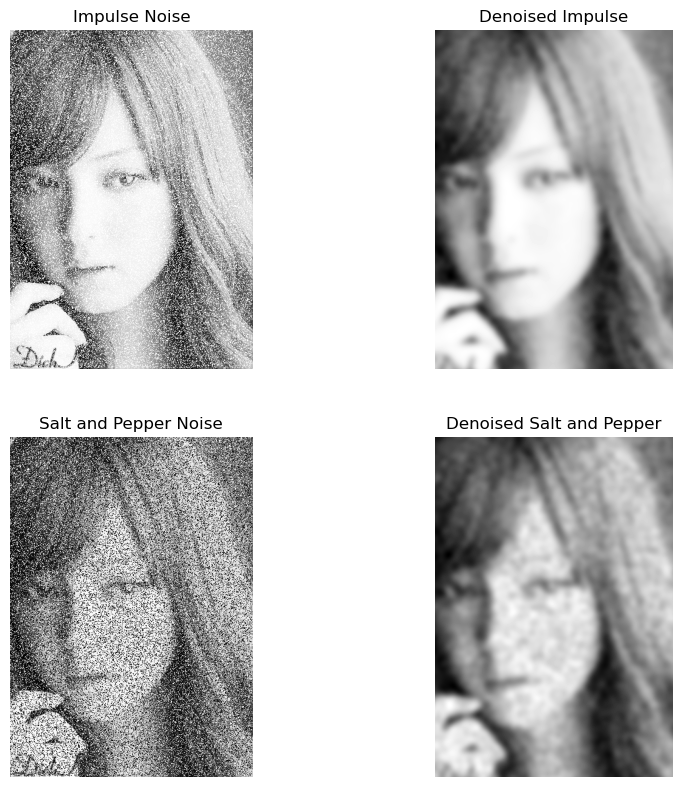
\includegraphics[width = 0.9\linewidth]{download (10).png}
        \caption{Bộ lọc Gauss tỏ ra kém hiệu quả trước các nhiễu đặc biệt}
        \label{fig10}
    \end{figure}  

    \subsection{Median-Filter}
    Ta thấy rằng bộ lọc Gauss đã không giải quyết triệt để được vấn đề khử nhiễu, cho nên bộ lọc \textit{Median} ra đời để xử lí điều đó.
    \\ \\ Trong thống kê, khi thu thập một lượng mẫu lớn về một sự kiện nào đó, việc đầu tiên nghĩ đến sẽ là lấy giá trị trung bình của chúng - đây chính xác là ý tưởng của \textit{Gaussian Filter}. Tuy nhiên, có một số trường hợp, người ta kị sử dụng giá trị trung bình, đó là khi số liệu có tính phân hóa cao. Khi đó thì \textit{Median} sẽ được sử dụng thay cho \textit{kì vọng}. \\ \\
    Có thể lấy ví dụ như sau:\\
    \fbox{
    \begin{minipage}{\textwidth}"Có một bạn sinh viên đi thi vấn đáp môn `Thị giác máy tính' trước hội đồng gồm 9 thầy cô. Sau khi đi thi số điểm bạn ấy nhận được lần lượt là 0, 0, 1, 2, 7, 8, 9, 10, 10. Điểm thì chỉ có một đầu điểm. Vậy có thể cho rằng bạn ý sẽ được bao nhiêu điểm?"
    \end{minipage}}
    \\ \\Dễ thấy rằng nếu tính theo kì vọng, số điểm trung bình của bạn sẽ là 5.2. Nhưng có vẻ sẽ không hợp lí lắm, khi phần lớn thầy cô đều cho bạn điểm khá cao. Trong trường hợp này, ta sử dụng trung vị (\textit{Median}) số điểm của bạn ấy có thể sẽ là 7 thì hợp lí hơn nhiều!    \\
    \textit{Tham khảo thêm tại} \href{https://vi.wikipedia.org/wiki/S%E1%BB%91_trung_v%E1%BB%8B}{Trung vị, wikipedia}
    \begin{figure}[ht!]
        \centering
        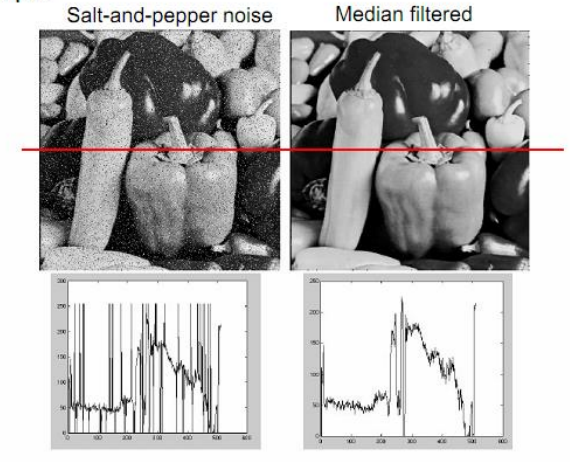
\includegraphics[width = 0.6\linewidth]{median.png}
        \caption{Lược đồ xám và ảnh. Sử dụng bộ lọc \textit{Median}}
        \label{fig11}
    \end{figure} \\  \\
    Hình \ref{fig11} cho ta minh họa về phép lọc \textit{Median}, ta thấy lược đồ xám của ảnh gốc, rất rất `lệch'. Sau khi sử dụng bộ lọc, kết quả hoàn toàn khiến chúng ta bất ngờ!\\
    \textbf{Tuy nhiên}, ảnh ta vẫn không tránh khỏi việc bị mờ đi nhiều so với ảnh gốc! Kernel size càng lớn, khử nhiễu càng tốt, nhưng ảnh càng làm mờ ảnh!
    \begin{figure}[ht!]
        \centering
        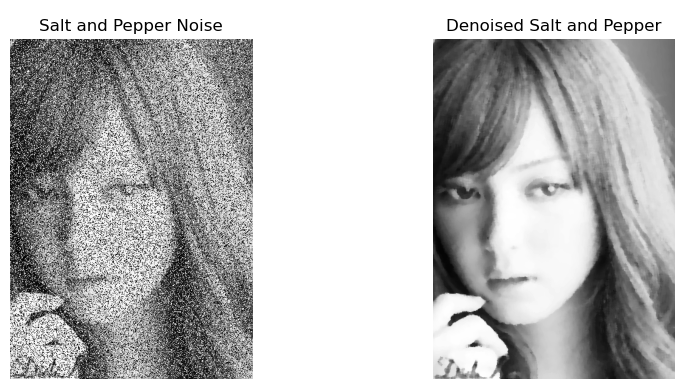
\includegraphics[width = \linewidth]{download (11).png}
        \caption{Mờ! Tác dụng phụ của \textit{Median Filter}}
        \label{fig11_}
    \end{figure} \\  
    \section{Sharpening Spatial Filters}
    \subsection{Đạo hàm bậc 1 và Đạo hàm bậc 2}
    Chúng ta đã không còn xa lạ với khái niệm đạo hàm, khái niệm mà hầu như ta dùng đến ở mọi lĩnh vực. Ý nghĩa của đạo hàm của một hàm số, ngoài cho ta biết về độ dốc, còn cho ta biết về hướng tăng của hàm số đó!\\
    Xuất phát từ định nghĩa:
    $$ f'(x) = \frac{f(x+\Delta) - f(x)}{\Delta}, \Delta \approx 0$$
    Trong hàm số liên tục, $\Delta$ là lân cận của x, tuy nhiên trong ảnh lân cận của một điểm ảnh chính là điểm ảnh ngay sát nó.\\ 
    Ta định nghĩa đạo hàm cho trường hợp rời rạc:
    $$ \frac{\partial f(x)}{\partial x} = f(x+1) - f(x)$$
    Trên là đạo hàm phải, mang ý nghĩa là nhìn về phía trước.
    Tương tự, ta có định nghĩa đạo hàm bậc hai cho trường hợp rời rạc:
    $$ \frac{\partial^2 f(x)}{\partial x^2} = f(x+1) + f(x-1) - 2f(x)$$
    hoàn toàn dễ suy ra từ khai triển \textit{Taylor}
    %\subsection{Gradient và Gradient của ảnh}
    %\textit{Gradient} là một khái niệm không xa lạ trong mạng \textit{Neural network} với \textit{Gradient descent}, hiểu đơn giản hơn, gradient mang dáng dấp của toán tử đạo hàm quen thuộc, mang ý nghĩa phản ánh hướng tăng của hàm số từ một điểm cho trước.
    %\\ \\ \textit{Gradient} của một hàm số $f(\textbf{x}): \mathbb{R}^n, \rightarrow \mathbb{R}$, được kí hiệu là $\nabla_{x} f(x)$, và:
    %$$ \nabla_{x} f(x) = \begin{bmatrix}
     %   \frac{\partial f}{\partial x_1} \\
      %  \frac{\partial f}{\partial x_2} \\
      %  \vdots \\
       % \frac{\partial f}{\partial x_n}
        %\end{bmatrix}$$
    %trong đó $\frac{\partial f}{\partial x_i}$ là đạo hàm riêng của hàm số theo thành phần thứ \textit{i}
    \subsection{Toán tử Laplace - Laplacian operator}
    Toán tử \textit{Laplace} được định nghĩa, như sau:
    $$ \nabla^2f = \frac{\partial^2 f}{\partial x^2} + \frac{\partial^2 f}{\partial y^2}$$
    Trong trường hợp rời rạc:
    $$ \nabla^2f = f(x+1,y) + f(x-1,y) + f(x,y+1) + f(x,y-1) - 4f(x,y) $$
    Dựa vào đó, ta có các bộ lọc tương ứng:
    \begin{figure}[ht!]
        \centering
        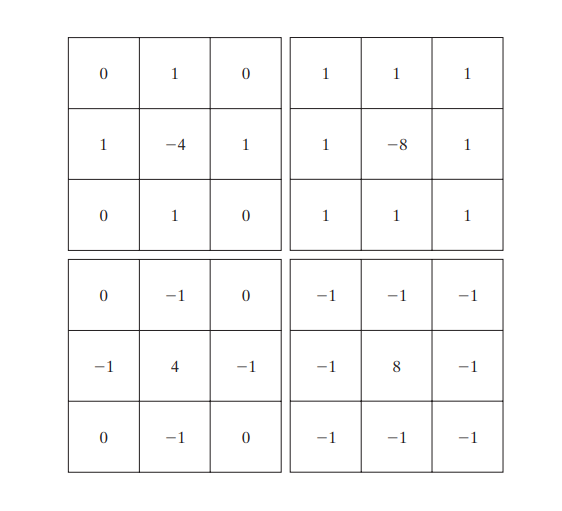
\includegraphics[width = 0.6\linewidth]{laplacian.png}
        \caption{Các bộ lọc Laplace, hai bộ lọc bên phải, là có tính cả đường chéo, khi đó hệ số của tâm sẽ là $\pm8$}
        \label{fig12}
    \end{figure}
    Hình \ref{fig12} minh họa về các bộ lọc \textit{Laplace}.
    \subsection{Làm nét ảnh bằng bộ lọc Laplace}
    \begin{equation}
        g(x,y) = f(x,y) + c \left[\nabla^2f(x,y) \right]
        \label{eq3}
    \end{equation}
    trong đó $c$ là hằng số, hoặc là 1 hoặc -1, phụ thuộc vào phần tử ở giữa bộ lọc. Xem lại mục (\ref{1}). \\
    Thật vậy, ta có nhận xét rằng, có thể kết hợp \ref{eq3} vào thành một bộ lọc!!! Ví dụ:
    $$
    \begin{bmatrix}
        0 & 1 & 0\\
        1  & -5 & 1\\
        0 & 1 & 0
    \end{bmatrix}
    \hspace{0.2\textwidth}
    \begin{bmatrix}
    1 & 1 & 1\\
    1 & -9 & 1 \\
    1 & 1 & 1
    \end{bmatrix}
    $$
    \begin{figure}[ht!]
        \centering
        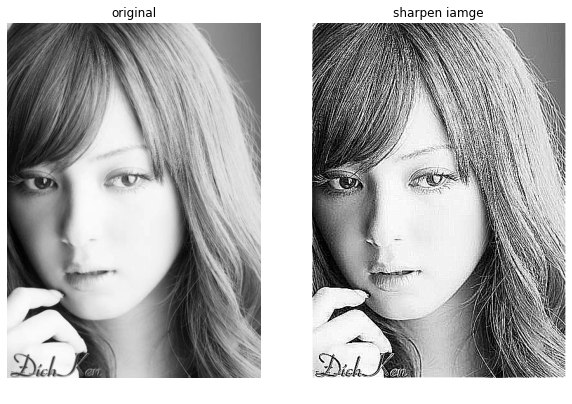
\includegraphics[width =\linewidth]{download (7).png}
        \caption{Kết quả với bộ lọc Laplace, sử dụng phiên bản kết hợp với bộ lọc chéo. cv2}
        \label{fig13}
    \end{figure}
    \subsection{Thảo luận}
    Tôi cũng như bạn, cũng thắc mắc tại sao lại có công thức (\ref{eq3}), tôi đã cố gắng suy nghĩ, và cũng có đôi chút suy đoán.\\
    Trước tiên, hãy nhìn vào Hình \ref{fig14}.
    \begin{figure}[ht!]
        \centering
        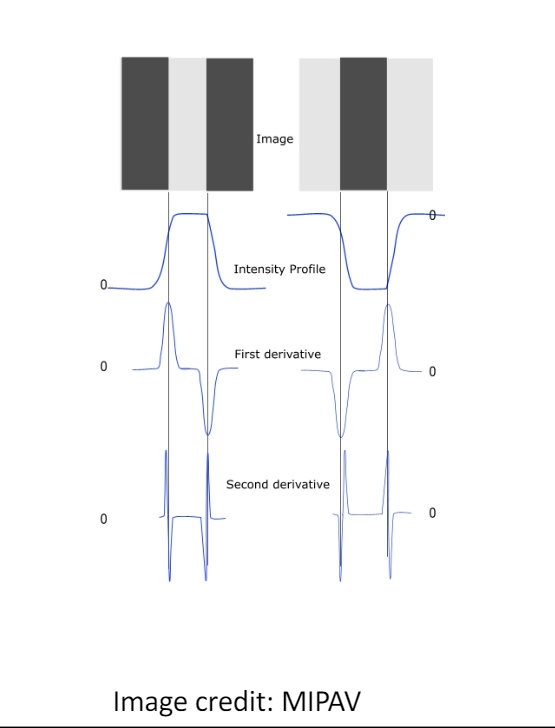
\includegraphics[width =0.9\linewidth]{download (6).png}
        \caption{Đạo hàm cấp một, cấp hai.}
        \label{fig14}
    \end{figure}
    \\ Những điểm có mức sáng thay đổi đột ngột sẽ là cạnh (\textit{edges}). Và nó sẽ ứng với vị trị mà đạo hàm bậc nhất đạt cực đại, hay đạo hàm bậc hai đạt 0. Qua toán tử đạo hàm, nhưng điểm có mức sáng bằng nhau sẽ bị chuyển về 0, tương tự với đạo hàm bậc 2.
    \\ Do đó nếu ta lấy ảnh gốc trừ đi ảnh đạo hàm cấp hai, cạnh và các điểm lân cận cùng mức sáng sẽ không thay đổi, nhưng lân cận của cạnh, sẽ càng tương phản. Dẫn đến ta trông ảnh ta như sắc nét hơn!
    \\ \textbf{Tuy nhiên}, toán tử của ta là toán tử \textit{Laplace} với việc cộng hai đạo hàm riêng nên suy luận trên cũng không hoàn toàn đúng!
    \\ \\
    Đó là lí thuyết nhưng trong thực tế:
    \begin{enumerate}
        \item Các điểm lân cận, dù gần nhau nhưng qua toán tử đạo hàm, điểm ảnh mới chưa chắc đã bằng 0. Lí do này khiến ảnh bị `\emph{tối hơn}' nếu sử dụng công thức (\ref{eq3}).
        \item Nếu không sử dụng toán tử kết hợp, mà sử dụng công thức (\ref{eq3}) thì rất dễ gây ra sai sót, bởi bộ lọc \textit{Laplace} không đảm bảo về tính trung bình của điểm ảnh (\textit{tổng các phần tử khác 1}).
    \end{enumerate}
    Để khắc phục điều này, có hai cách:
    \begin{enumerate}
        \item Chuẩn hóa ảnh sau khi dùng toán tử \textit{Laplace} rồi nhân với 255 làm tròn. Trước khi dùng công thức (\ref{eq3}). Nếu ảnh tối thì ta có thể làm sáng lại bằng các phương pháp của bài trước!
        \item Dùng thẳng công thức thu gọn, kết hợp với hàm \emph{filter2D} của thư viện \emph{cv2}.
        \item Trong trường hợp muốn dùng hằng số $c$ khác 1, -1 thì đừng quên mục \ref{1}
    \end{enumerate}
    \begin{figure}[ht!]
        \centering
        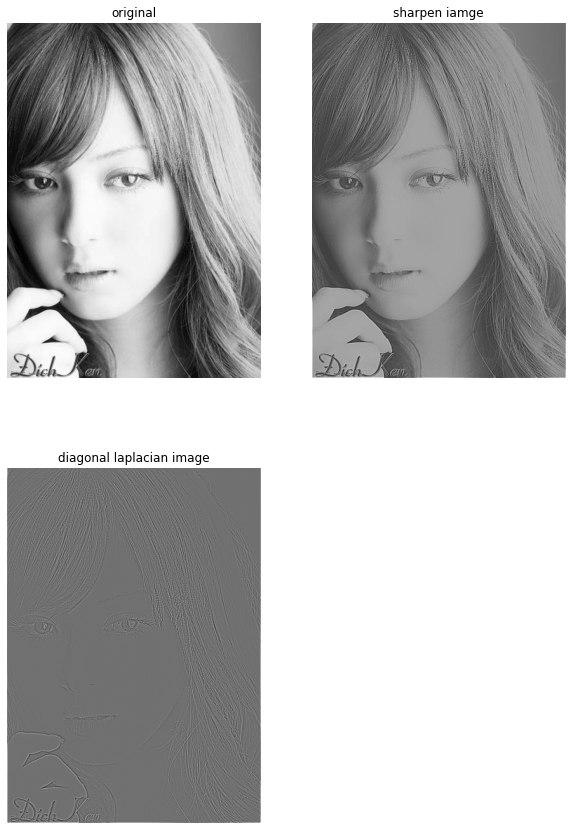
\includegraphics[width =0.9\linewidth]{download (8).png}
        \caption{Phỏng theo lí thuyết, tuy nhiên chưa quá hiệu quả.}
        \label{fig15}
    \end{figure}
    Tuy nhiên những khắc phục này chưa triển để. Hình \ref{fig15}. Và trong việc này thư viện \textit{cv2} làm tốt hơn, so với tự làm theo lí thuyết!
    \\ \\
    Ngoài cách làm nét này bạn có thể tham khảo thêm \textit{Highboost Filtering} cũng khá tương tự.
    \section{Mã nguồn}
    Mã nguồn của bài này có thể tham khảo tại đây:
    \href{https://github.com/thuantn210823/Computer-Vision-IPSAL-LAB-}{ \textit{My Github}}
    , \href{https://colab.research.google.com/drive/1OJPnCVz51zampZyWqOYpRambrDB2h50P#scrollTo=qPMVzpSSz6Ft}{\textit{Link colab}}
    Tuy nhiên phần làm nét tôi không làm tốt cho lắm, ảnh ở đây là vừa làm lại để đối chiếu, trong mã nguồn trên sẽ không có!\\
    Trong bài tới ta sẽ đi sâu hơn về việc xác định cạnh!
    
    %\section{Báo cáo}
    \newpage
    \section{Tài liệu tham khảo}
    \begin{thebibliography}{9}
    \bibitem{slide}
    Truong. PV, Thao. TT \emph{Silde bài giảng tuần 4}, Đại học Bách Khoa Hà Nội.
    \bibitem{book}
    R.C. Gonzalez and R.E. Woods \emph{Digital image processing ($3^{rd}$ editon)}, Prentice Hall, 2008.
    \bibitem{website}
    Tiep. VK \href{https://machinelearningcoban.com/2018/10/03/conv2d}{Bài 37: Tích chập hai chiều}, machinelearningcoban.com, 2018.
    \bibitem{website}
    D2l \href{https://d2l.aivivn.com/chapter_convolutional-neural-networks/conv-layer_vn.html}{6.2 Phép tích chập cho ảnh}, d2l.aivivn.com. 
    \bibitem{website}
    \url{https://viblo.asia/p/tuan-5-gradient-and-edge-bJzKmOGwl9N}
    \bibitem{website}
    Wikipedia \href{https://vi.wikipedia.org/wiki/S%E1%BB%91_trung_v%E1%BB%8B}{Trung vị}
    \bibitem{website}
    Wikipedia \href{https://en.wikipedia.org/wiki/68%E2%80%9395%E2%80%9399.7_rule}{Three sigma rule}
    \end{thebibliography}
\end{document}
